\begin{mdframed}[style=warning]
	\begin{ejercicio}
		\textbf{Conceptos.}
		\begin{enumerate}
			\item Si $\vec{A}$ y $\vec{B}$ son vectores distintos de cero, ¿es posible que $\vec{A} \cdot \vec{B}$ y $\vec{A} \cp \vec{B}$? Explique.
			\item Muestre que sin importar lo que sean $\vec{A}$ y $\vec{B}$, $\vec{A} \cdot \qty(\vec{A} \cp \vec{B}) = 0$.
		\end{enumerate}
	\end{ejercicio}
\end{mdframed}









\begin{mdframed}[style=warning]
	\begin{ejercicio}
		Dados los vectores $\vec{A}$ y $\vec{B}$, con un ángulo $\theta$ entre ellos demuestre, utilizando el producto punto, que la magnitud del vector resultante $\vec{R}$ de la suma $\vec{A} + \vec{B}$ es
			$$ R = \sqrt{A^2 + B^2 + 2AB\cos{\theta}} $$
		donde $A$ y $B$ son las magnitudes $\vec{A}$ y $\vec{B}$.
	\end{ejercicio}
\end{mdframed}







\begin{mdframed}[style=warning]
	\begin{ejercicio}
	Resuelva los siguientes incisos.
		\begin{itemize}
			\item Encuentre el ángulo entre las diagonales de las caras contigüas de un cubo.
			\begin{center}
				


\tikzset{every picture/.style={line width=0.75pt}} %set default line width to 0.75pt        

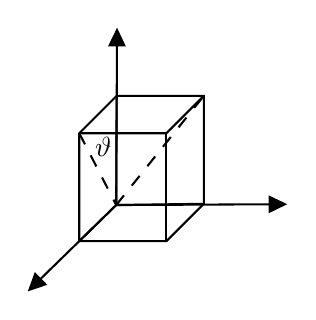
\begin{tikzpicture}[x=0.75pt,y=0.75pt,yscale=-1,xscale=1]
%uncomment if require: \path (0,300); %set diagram left start at 0, and has height of 300

%Shape: Cube [id:dp6038747680393932] 
\draw   (350,136) -- (368,118) -- (410,118) -- (410,170) -- (392,188) -- (350,188) -- cycle ; \draw   (410,118) -- (392,136) -- (350,136) ; \draw   (392,136) -- (392,188) ;
%Straight Lines [id:da6829094301047849] 
\draw    (368,118) -- (367.8,170.6) ;
%Straight Lines [id:da36124944068918086] 
\draw    (367.8,170.6) -- (410,170) ;
%Straight Lines [id:da004458006903363065] 
\draw    (367.8,170.6) -- (350,188) ;
%Straight Lines [id:da21943316361290965] 
\draw  [dash pattern={on 4.5pt off 4.5pt}]  (367.8,170.6) -- (410,118) ;
%Straight Lines [id:da569309436281727] 
\draw  [dash pattern={on 4.5pt off 4.5pt}]  (350,136) -- (367.8,170.6) ;
%Straight Lines [id:da7593701970272995] 
\draw    (367.8,170.6) -- (368.19,88.2) ;
\draw [shift={(368.2,85.2)}, rotate = 90.27] [fill={rgb, 255:red, 0; green, 0; blue, 0 }  ][line width=0.08]  [draw opacity=0] (8.93,-4.29) -- (0,0) -- (8.93,4.29) -- cycle    ;
%Straight Lines [id:da0012548071934168625] 
\draw    (367.8,170.6) -- (447.2,170.21) ;
\draw [shift={(450.2,170.2)}, rotate = 179.72] [fill={rgb, 255:red, 0; green, 0; blue, 0 }  ][line width=0.08]  [draw opacity=0] (8.93,-4.29) -- (0,0) -- (8.93,4.29) -- cycle    ;
%Straight Lines [id:da2187449744897081] 
\draw    (367.8,170.6) -- (327.35,210.1) ;
\draw [shift={(325.2,212.2)}, rotate = 315.68] [fill={rgb, 255:red, 0; green, 0; blue, 0 }  ][line width=0.08]  [draw opacity=0] (8.93,-4.29) -- (0,0) -- (8.93,4.29) -- cycle    ;

% Text Node
\draw (356.2,136.6) node [anchor=north west][inner sep=0.75pt]    {$\vartheta $};


\end{tikzpicture}

			\end{center}
			\pagebreak
			\item Encuentre el ángulo mostrado en la figura.
			\begin{figure}[H]
				\centering
				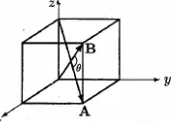
\includegraphics[scale=0.5]{./img/cube.png}
			\end{figure}
		\end{itemize}
	\end{ejercicio}
\end{mdframed}






\begin{mdframed}[style=warning]
	\begin{ejercicio}
		\begin{multicols}{2}
		Utilice el producto cruz para encontrar las componentes del vector unitario $\vu{n}$ perpendicular a una de las caras del tetraedro de la siguiente figura:
		\columnbreak
		\begin{figure}[H]
			\centering
			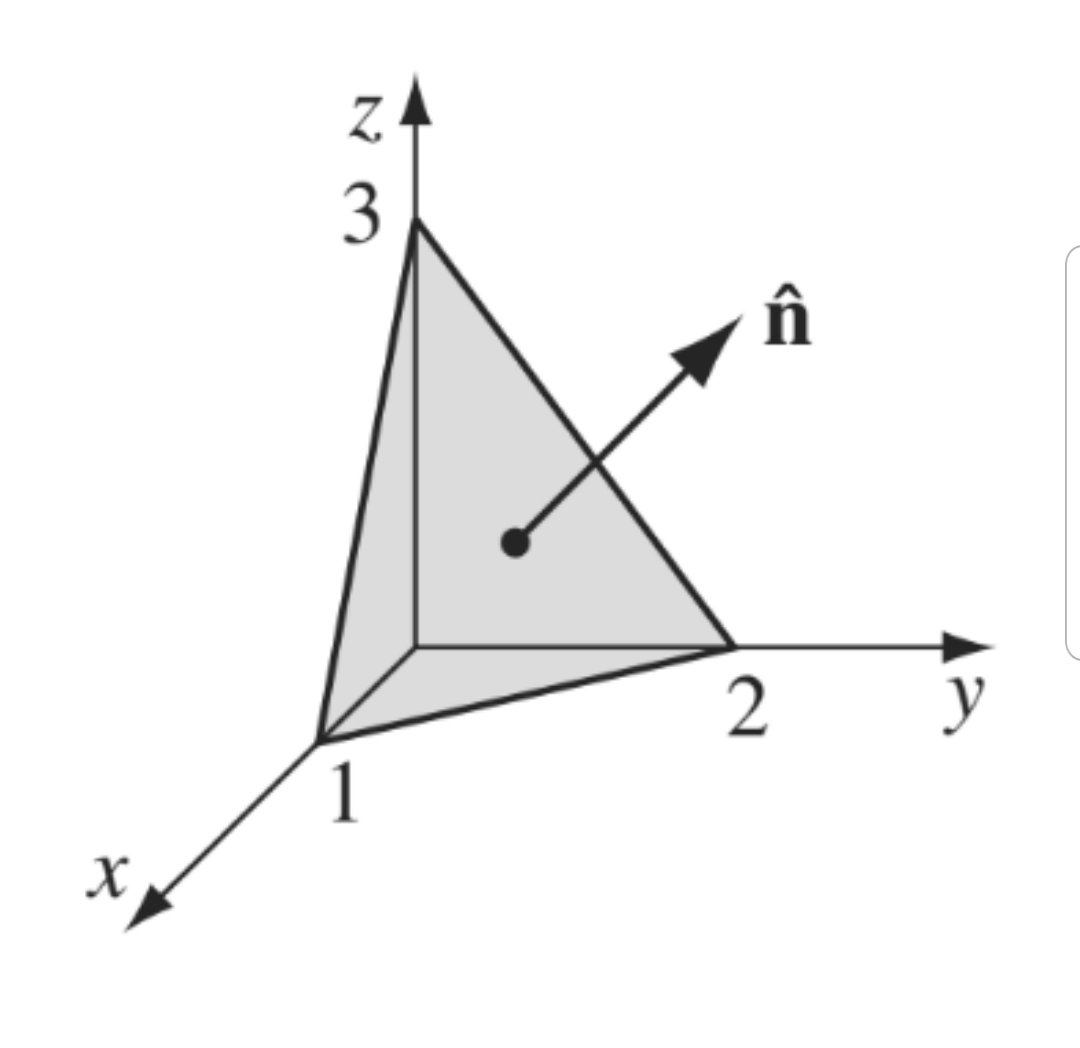
\includegraphics[scale=0.07]{./img/tetraedro.jpeg}
			\caption{Tetraedro.}
			\label{tetraedro}
		\end{figure}
		\end{multicols}
	\end{ejercicio}
\end{mdframed}

















































%%%